% Drawing 76/01-4 -- folder 76, batch 01, archive page 12 (PDF page 13).
% Transcription: figure : un graphe, deux sommets cerclés reliés par une longue arête ; au premier pendent trois arêtes courtes ; le second, cerclé en bas, porte deux arêtes marquées d'un point milieu et une arête vers un troisième sommet cerclé, d'où partent trois arêtes formant un fuseau
% Kind: graph with ringed vertices and a spindle. Method 2 (schematic redraw from the facsimile). Status: ok.
% Notes: A ringed vertex with three short pendant edges, joined by a long arc to the right; a ringed vertex below carries two edges marked by a middle point and an edge (also with a middle point) to a vertex from which three edges form a spindle ending in a third ringed vertex at the top right. On the page the spindle starts from an unringed vertex and ends in the ringed one (the transcription puts the ring at the start).
% Coordinates: 1 unit = 1 mm = 1/100 of the crop width (bbox in page fractions: [0.58, 0.15, 0.93, 0.3]).
% Redrawn by Claude (claude-opus-5-5), issue #73, 2026-11-07; not checked by a human; not compiled (no TeX in the session).
% Rights: reproduces part of the work -- behind RENDER_TRANSCRIPTS, never published by itself.
\documentclass[tikz,border=3pt]{standalone}
\usepackage{amsmath,amssymb}
\usetikzlibrary{patterns,arrows.meta}
\tikzset{pencil/.style={black!45}, struck/.style={black!35}, mark/.style={circle,draw,inner sep=1.3pt}, pt/.style={circle,fill,inner sep=0.9pt}, opt/.style={circle,draw,fill=white,inner sep=1.1pt}}
\begin{document}
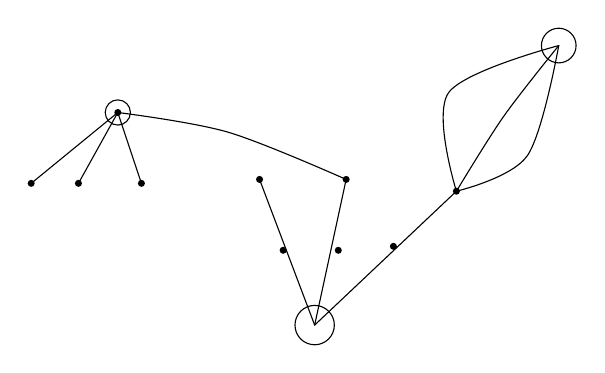
\begin{tikzpicture}[x=1mm,y=1mm,line cap=round,line join=round,font=\scriptsize]
\draw (21,-28.5) circle[radius=1.6];
\node[pt] at (21,-28.5) {};
\draw (21,-28.5) -- (10,-37.5);
\draw (21,-28.5) -- (16,-37.5);
\draw (21,-28.5) -- (24,-37.5);
\node[pt] at (10,-37.5) {};
\node[pt] at (16,-37.5) {};
\node[pt] at (24,-37.5) {};
\draw plot[smooth, tension=0.55] coordinates {(21,-28.5) (35,-31) (50,-37)};
\draw (46,-55.5) circle[radius=2.5];
\node[pt] at (39,-37) {};
\node[pt] at (50,-37) {};
\draw (39,-37) -- (46,-55.5);
\draw (50,-37) -- (46,-55.5);
\node[pt] at (42,-46) {};
\node[pt] at (49,-46) {};
\draw (46,-55.5) -- (64,-38.5);
\node[pt] at (56,-45.5) {};
\node[pt] at (64,-38.5) {};
\draw plot[smooth, tension=0.55] coordinates {(64,-38.5) (63,-26) (77,-20)};
\draw plot[smooth, tension=0.55] coordinates {(64,-38.5) (70,-29) (77,-20)};
\draw plot[smooth, tension=0.55] coordinates {(64,-38.5) (73,-34) (77,-20)};
\draw (77,-20) circle[radius=2.2];
\end{tikzpicture}
\end{document}
